\subsection{A small bump}
On June 2nd 2015, the day before CMS recorded its first ever 13 TeV event, a pre-print appeared on the arXiv "Search for high-mass diboson resonances with boson-tagged jets in proton-proton collisions at $\sqrt{s} = 8$ \TeV with the ATLAS detector"~\cite{Aad2015}.
It was an analysis of the full ATLAS Run 1 dataset, corresponding to 20.3 \fbinv, searching for heavy resonances decaying to vector bosons in the all-hadronic state. The analysis documented a 3.4 $\sigma$ excess for a heavy resonance decaying to \PW\PZ around 2 \TeV.
The corresponding CMS analysis, published the previous year, had a 1.3 $\sigma$ excess at roughly the same resonance mass, but mostly compatible with a \PW\PW final state hypothesis~\cite{Khachatryan:1700394}. Figure~\ref{fig:searchI:8tev} shows the corresponding dijet invariant mass spectrum as seen by ATLAS (left) and the upper limit on the production times the cross section for a $G_{Bulk}$ decaying to \PW\PW (right)  as documented by CMS.

\begin{figure}[ht] 
    \centering
    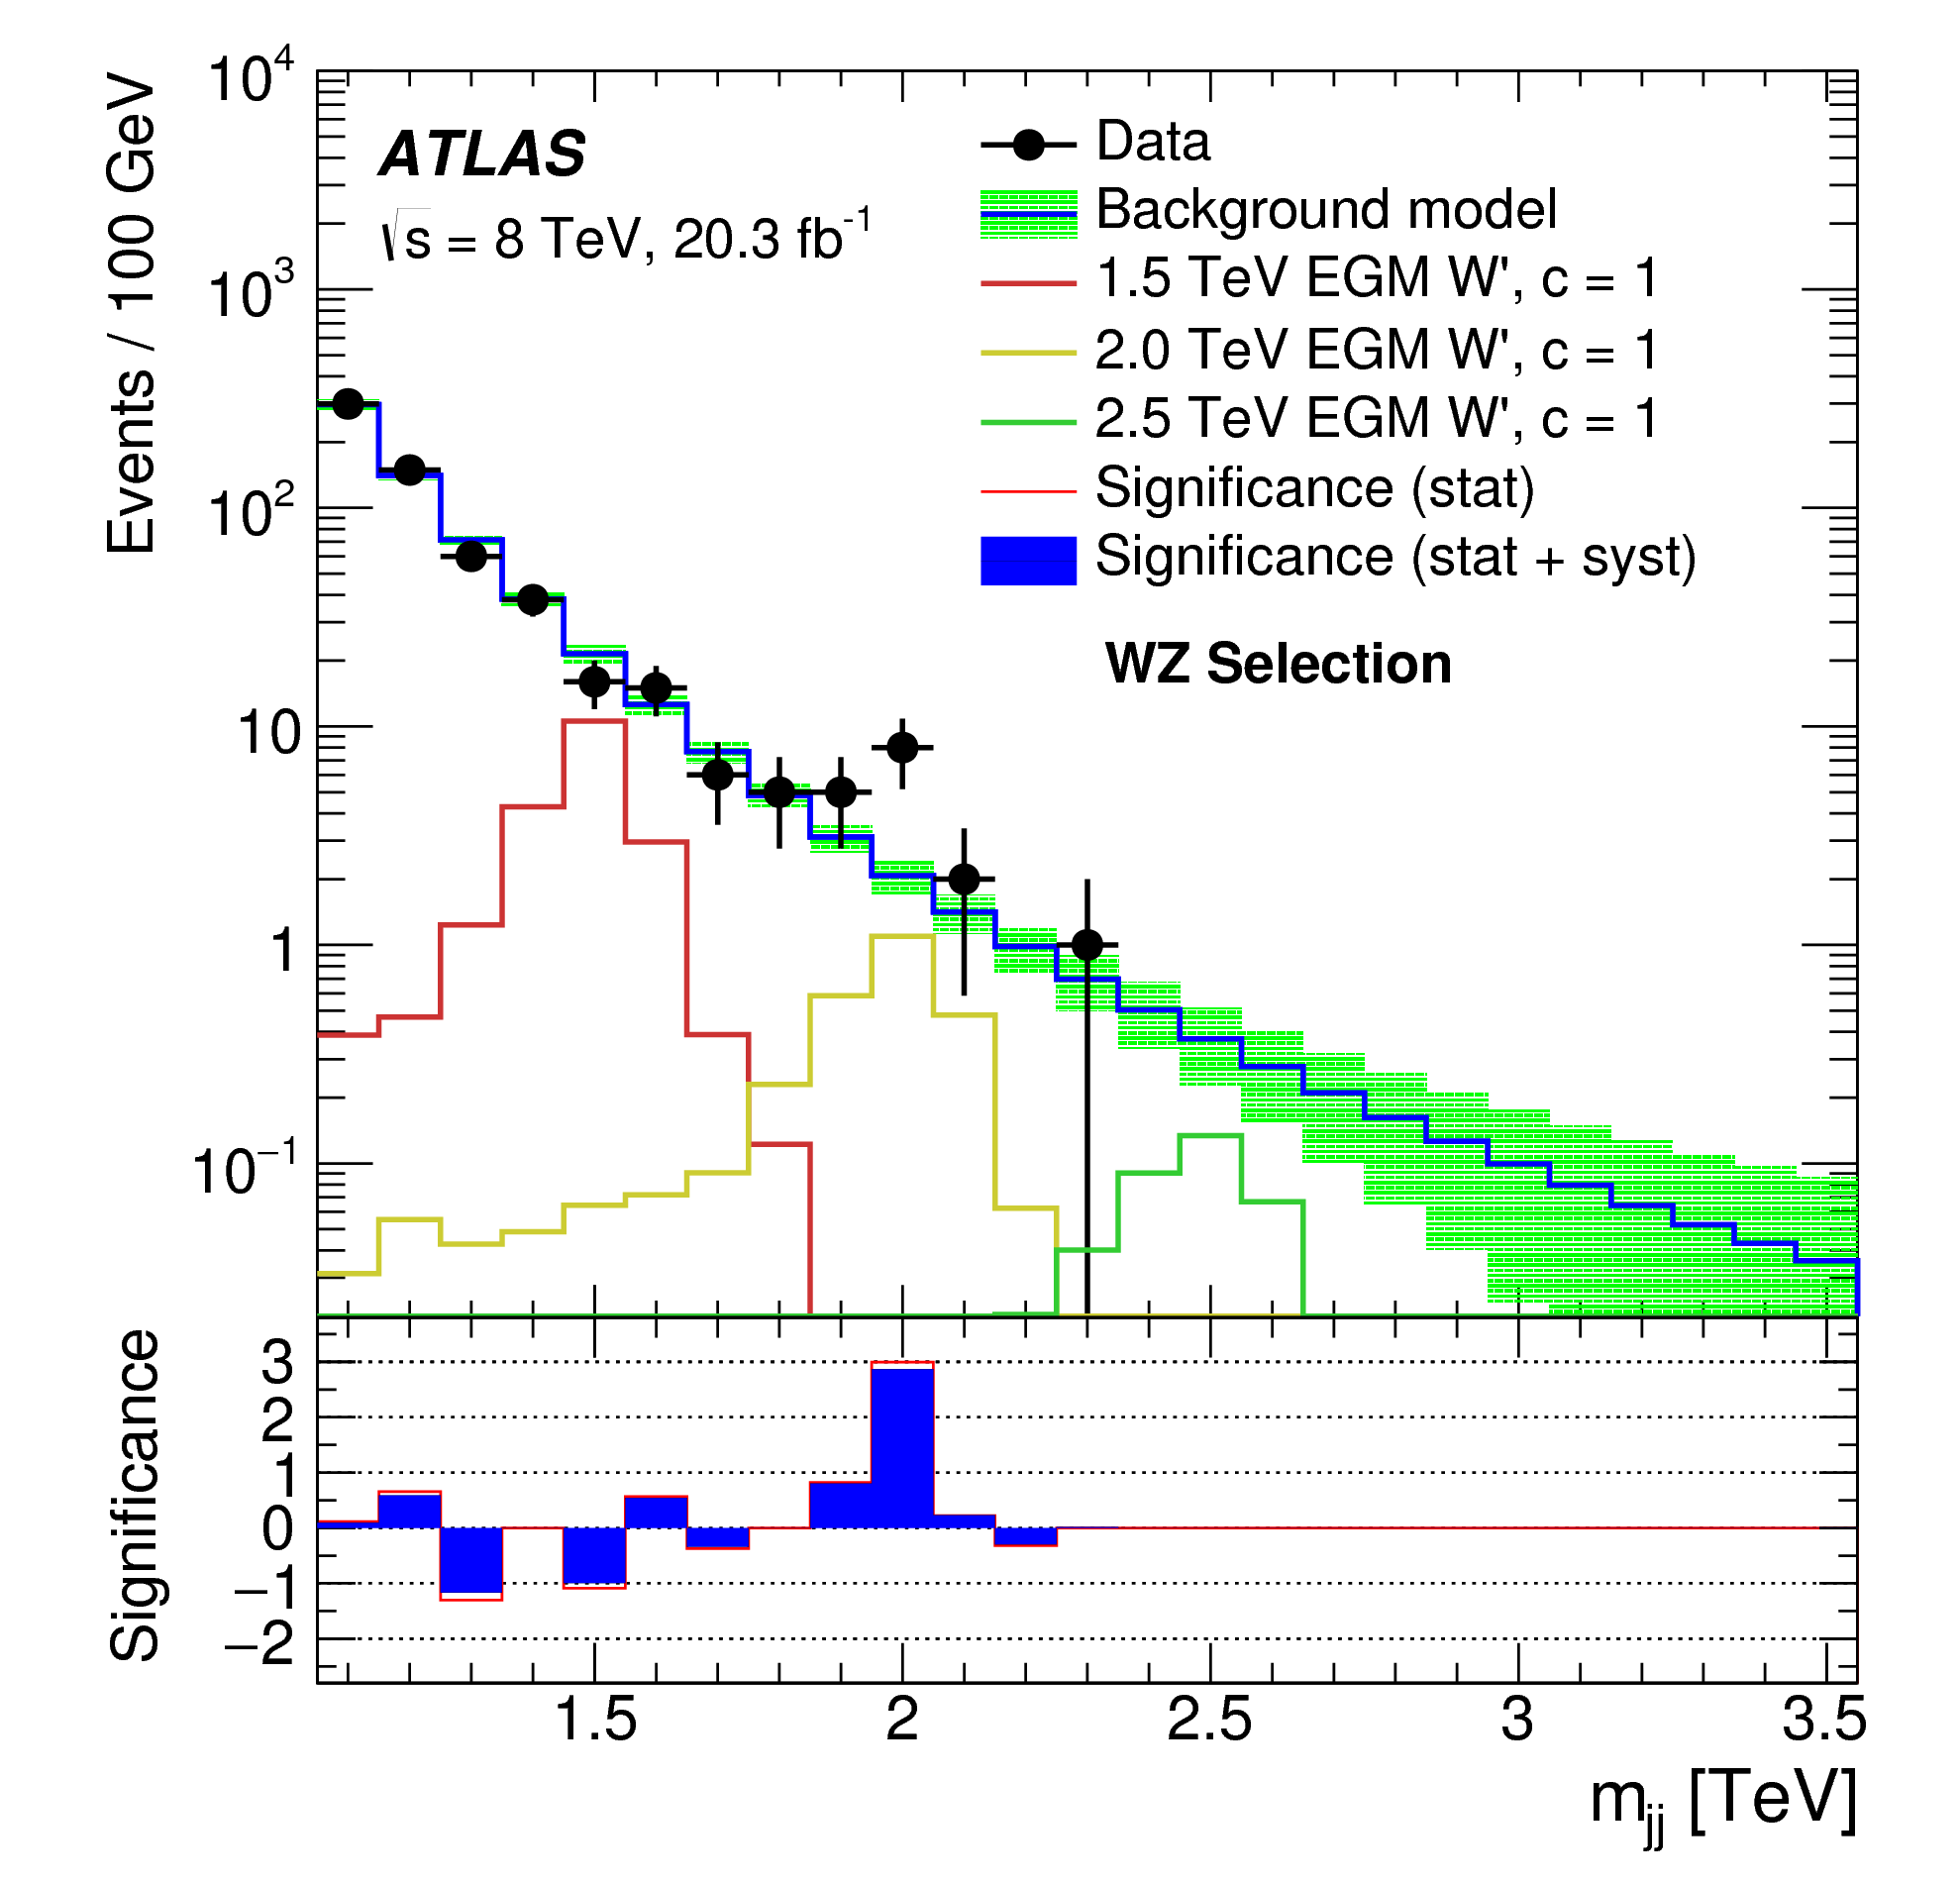
\includegraphics[width=0.4\textwidth]{figures/analysis/search1/misc/atlas_8tev.png}
    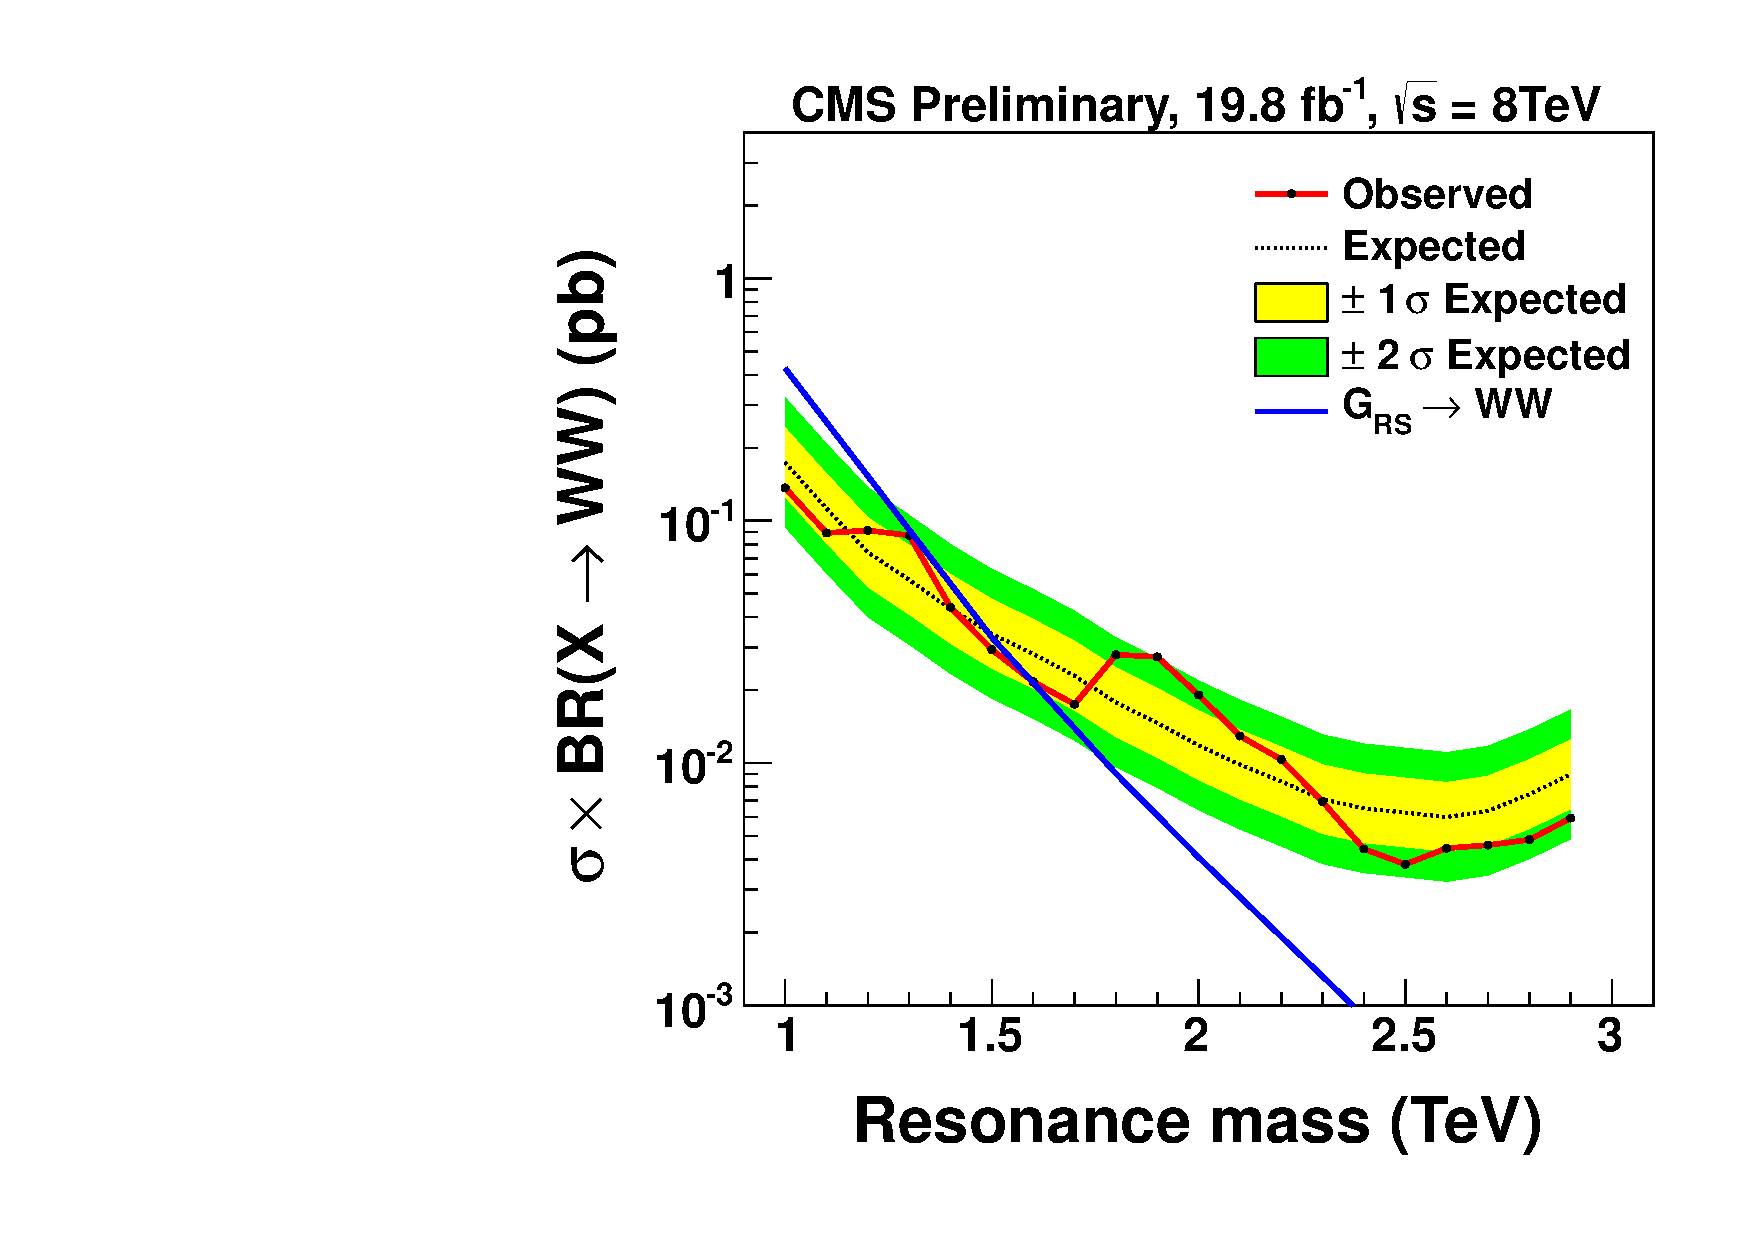
\includegraphics[width=0.4\textwidth]{figures/analysis/search1/misc/EXO-12-024_gWW.pdf}
    \caption{The mass (top) and \PT (bottom) resolution comparing PF only (blue), PF+CHS (red) and PUPPI (pink) jets. The absolute resolution (left) as well as the resolution as a function of the number of reconstructed primary vertices in the event (right)is shown~\cite{Bertolini2014}.}
    \label{fig:searchI:8tev}
\end{figure}

The two measurements were found to be compatible, favoring a heavy resonance with a production cross section of around 5 \fbinv and a mass between 1.9 and 2.0 TeV decaying to either \PW\PW, \PW\PZ or \PZ\PZ~\cite{Dias:2015mhm}. Figure~\ref{fig:searchI:8tevcombo} show the obtained p-value of the ATLAS (red) and CMS (blue) search as well as their combination (black).  

\begin{figure}[ht] 
    \centering
    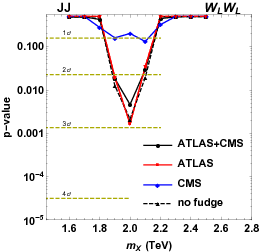
\includegraphics[width=0.25\textwidth]{figures/analysis/search1/misc/CMS_ATLAS_BulkWW_JJ_dijetfit_p.png}
    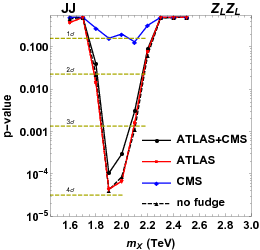
\includegraphics[width=0.25\textwidth]{figures/analysis/search1/misc/CMS_ATLAS_BulkZZ_JJ_dijetfit_p.png}
    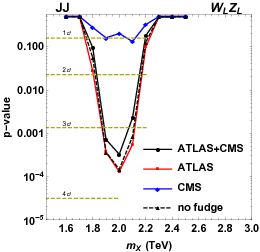
\includegraphics[width=0.25\textwidth]{figures/analysis/search1/misc/CMS_ATLAS_WZ_JJ_dijetfit_p.png}
    \caption{p-values as a function of resonance mass obtained with an emulation of the ATLAS (red) and CMS (blue) searches as well as the combination of the two (black). Here for a \PW\PW (left), \PW\PZ (middle) and \PZ\PZ (right) hypothesis~\cite{Dias:2015mhm}.}
    \label{fig:searchI:8tevcombo}
\end{figure}

The combination of the two excesses and the timing of the ATLAS paper, naturally lead to quite a commotion. And in the coming weeks, the arXiv was flooded with theory papers seeking an explanation for measurements.
The pressure on seeing early results with 13 TeV data in the VV all-hadronic final state was high, and it was agreed with CMS Physics Coordination that a preliminary analysis would be ready in December that same year.

\subsection{Analysis strategy}

When a resonance X with a mass above 1 TeV decays into a vector boson pair, the bosons have a very high energy ($\tilde\PT=\mX/2=500 \GeV$, assuming X is produced at rest). The boson is co-called "boosted".
The decay products of a hadronically decaying boosted vector boson, will therefore not appear as back-to-back in the lab frame but rather be very collimated, as described in Section~\ref{sec:objreco:substructure}.

\subsection{Event selection}

